\documentclass[black,white]{beamer}
\usepackage{beamerthemesplit}
\usepackage{amsmath}
\usepackage{hyperref}
\usepackage{listings}
\usepackage{lmodern}
\usepackage{tikz}
\usepackage{hyperref}
\usepackage{listings}
\usepackage{lmodern}
\usepackage{pifont}
\usepackage{svg} % Requires inkscape
\usepackage{tikz}
\usetikzlibrary{mindmap}
\usepackage{verbatim}

\beamertemplatenavigationsymbolsempty
\usecolortheme{dove}
\useoutertheme{infolines}
\useinnertheme{rectangles}

\newcommand{\cmark}{\ding{51}}%
\newcommand{\bigcmark}{{\large\textcolor{green}\cmark}}
\newcommand{\xmark}{\ding{55}}
\newcommand{\bigxmark}{{\large\textcolor{red}\xmark}}
\newcommand\blfootnote[1]{%
  \begingroup
  \renewcommand\thefootnote{}\footnote{#1}%
  \addtocounter{footnote}{-1}%
  \endgroup
}

\definecolor{ashgrey}{rgb}{0.7, 0.75, 0.71}
\definecolor{charcoal}{rgb}{0.21, 0.27, 0.31}
\definecolor{powderblue}{rgb}{0.69, 0.88, 0.9}
\definecolor{layerblue}{RGB}{213, 234, 254}
\newcommand\sectioncolor{\setbeamercolor{background canvas}{bg=layerblue}}

\title[BPF Socket Lookup]{Building socket-aware BPF programs}
\institute{Cilium.io}
\author[Joe Stringer]{Joe Stringer}

\setbeamertemplate{footline}
{
    \leavevmode%
    \hbox{%
        \begin{beamercolorbox}[wd=.333333\paperwidth,ht=2.25ex,dp=1ex,center]{author in head/foot}%
            \usebeamerfont{author in head/foot}\insertshortauthor
        \end{beamercolorbox}%
        \begin{beamercolorbox}[wd=.333333\paperwidth,ht=2.25ex,dp=1ex,center]{title in head/foot}%
            \usebeamerfont{title in head/foot}\insertshorttitle
        \end{beamercolorbox}%
        \begin{beamercolorbox}[wd=.333333\paperwidth,ht=2.25ex,dp=1ex,right]{date in head/foot}%
            \usebeamerfont{date in head/foot}\insertshortdate{}\hspace*{2em}
            \insertframenumber{} / \inserttotalframenumber\hspace*{2ex}
        \end{beamercolorbox}}%
        \vskip0pt%
}

\newcommand\newsectionpage[1]{
    \section{}
    {\sectioncolor
        \begin{frame}
            \vfill
            \centering
            \section{#1}
            \begin{beamercolorbox}[sep=8pt,center,shadow=true,rounded=true]{title}
                \usebeamerfont{title}\insertsectionhead\par%
            \end{beamercolorbox}
            \vfill
        \end{frame}
    }
    \section{#1}
}

\date[Nov 13, 2018]{Linux Plumbers 2018, Vancouver, BC}

\begin{document}
    {\sectioncolor
    \begin{frame}
    \titlepage
    \end{frame}
    }

    \begin{frame}{}
        \centering
        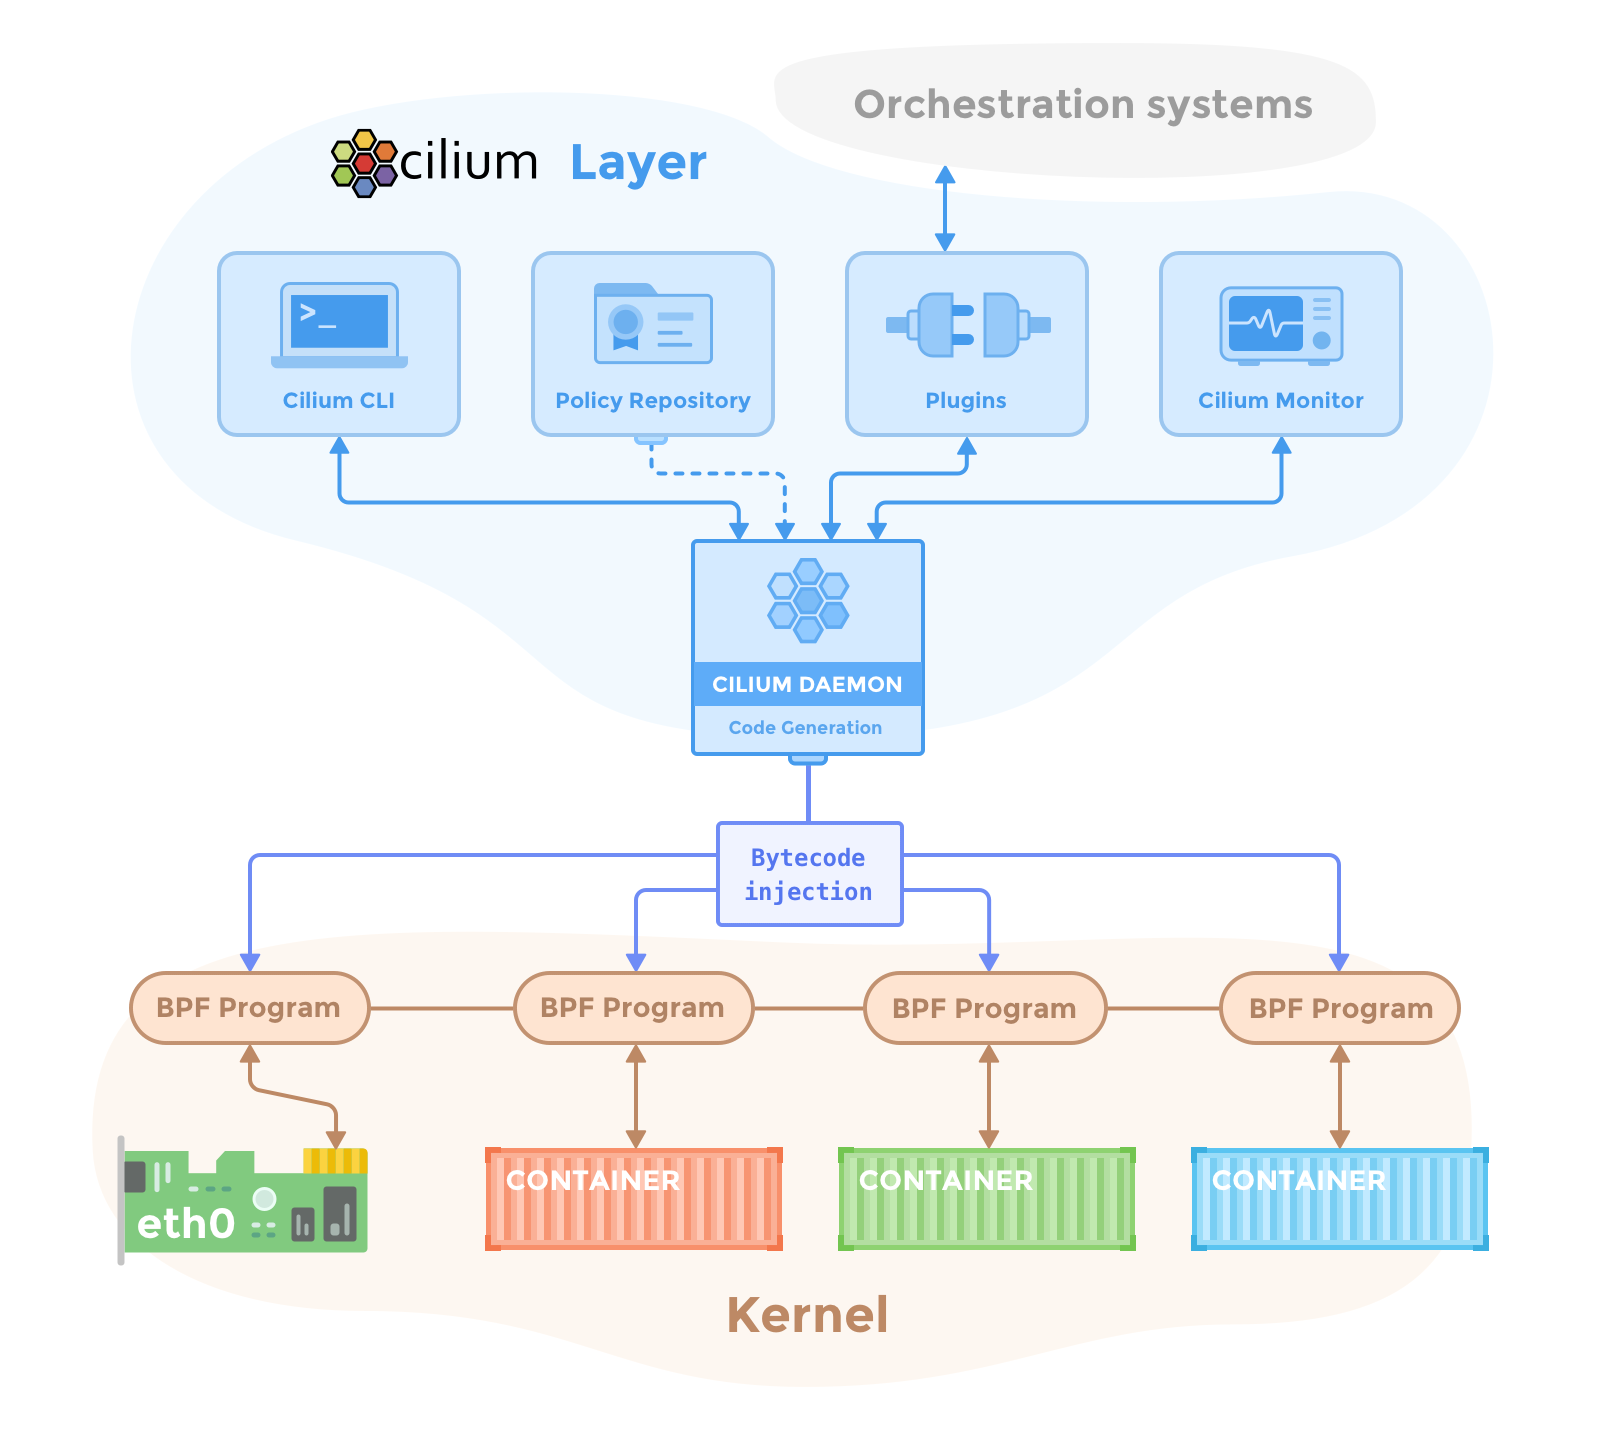
\includegraphics[width=0.8\textwidth]{cilium_architecture.png}
    \end{frame}

    \section{Background}

    % Why is this important?
    % Basic: Only allow legitimate replies
    % Advanced: Perform additional checks on the packet
    \begin{frame}{Network Policy}
        \begin{center}
        "Endpoint A can talk to endpoint B"% \smallskip
            \[\implies\]
        "Endpoint B can reply to endpoint A"
        \end{center}
    \end{frame}

    % Background: What have people been doing for stateful firewalling?
    %\begin{frame}{A (selective) history of traffic filtering}
    %    \begin{columns}[c]
    %        \begin{column}{0.15\textwidth}
    %            1992\\ \smallskip
    %            1994\\ \smallskip
    %            \ldots\\ \smallskip
    %            1999\\ \smallskip
    %            ~\\ \smallskip
    %            2002\\ \smallskip
    %            2005\\ \smallskip
    %            2008\\ \smallskip
    %            \ldots\\ \smallskip
    %            2014\\ \smallskip
    %        \end{column}
    %        \hspace{-50pt}
    %        \vrule{}
    %        \begin{column}{0.85\textwidth}
    %            %The Packet Filter (ACM SOSP)\\
    %            The BSD Packet Filter [McCanne, Jacobson]\\ \smallskip
    %            Stateful firewalls become commercially available\\ \smallskip
    %            ~\\ \smallskip
    %            Implementing a Distributed Firewall [Ioannidis {\em et al.}]\\ \smallskip
    %            Linux TC (upstream 2000), Netfilter (upstream 2001)\\ \smallskip
    %            BSD/OS IPFW [Lidl {\em et al.}]\\ \smallskip
    %            A model of stateful firewalls [Gouda, Liu]\\ \smallskip
    %            Linux Network Namespaces\\ \smallskip
    %            ~\\ \smallskip
    %            Linux gets Extended BPF\\ \smallskip
    %        \end{column}
    %    \end{columns}
    %\end{frame}

    %% What happens with BPF when first introduced?
    %\begin{frame}{Berkeley Packet Filter}
    %    \begin{itemize}
    %        \item Initial use case: network monitoring \medskip % Successor to CSPF
    %            \begin{itemize}
    %                \item Open socket \medskip
    %                \item Attach filter \medskip
    %                %\item Bob's your uncle
    %            \end{itemize}
    %        \item TCPdump becomes the de facto monitoring tool \medskip
    %        \item BPF remains stateless, and just for socket filtering
    %        %\item BSD/OS IPFW looked to extend this for other use cases
    %    \end{itemize}
    %\end{frame}

    % What does Linux do for firewalling?
    \begin{frame}[fragile]{How have we built these before?}
        \centering
        \vfill
        \includesvg[width=0.8\textwidth]{sfw-ct-policy.svg}
%        \begin{verbatim}
%      +-+    +--------------+    +--------------+
%+-----+      |  Connection  |    |    Policy    |
%| NIC +------>   Tracker    +---->              +---->
%+-----+      +--------------+    +--------------+
%        \end{verbatim}
        \vfill
    \end{frame}

    \begin{frame}[fragile]{Let's do this with BPF}
        \begin{itemize}
            \item Attach BPF to packet hook \bigcmark \medskip
            \item ``Connection Tracking'' BPF map \bigcmark \smallskip
            \begin{itemize}
                \item Key by 5-tuple \medskip
                \item Associate counters, NAT state, etc. \medskip
		        \item Handle tuple flipping \medskip
            \end{itemize}
            \item ``Policy'' map \bigcmark \medskip
            \item Deploy! \bigcmark \smallskip
            \begin{itemize}
                \item[] \medskip
                \item[] \medskip
                \item[] \medskip
            \end{itemize}
        \end{itemize}
    \end{frame}

    \begin{frame}[fragile]{Let's do this with BPF}
        \begin{itemize}
            \item Attach BPF to packet hook \bigcmark \medskip
            \item ``Connection Tracking'' BPF map \bigcmark \smallskip
            \begin{itemize}
                \item Key by 5-tuple \medskip
                \item Associate counters, NAT state, etc. \medskip
		        \item Handle tuple flipping \medskip
            \end{itemize}
            \item ``Policy'' map \bigcmark \medskip
            \item Deploy! \bigxmark \smallskip
            \begin{itemize}
                \item \verb+nf_conntrack: table full, dropping packet+ \medskip
                \item Hmm, how big should this map be again? \medskip
                \item How do we clean this up\ldots \medskip
            \end{itemize}
        \end{itemize}
    \end{frame}

    %\begin{frame}[fragile]{Recent trends: BPF comeback}
    %    \begin{itemize}
    %        \item Netfilter \verb+xt_bpf+ \medskip
    %        \item TC \verb+cls_bpf+ \medskip
    %        \item Open vSwitch \medskip
    %        \item eXpress Data Path \medskip
    %        \item BPFilter \medskip
    %    \end{itemize}
    %\end{frame}

    %\newsectionpage{Socket introspection from packet handlers}

    % What does Linux do for firewalling?
    \begin{frame}{Why model it like this?}
        \begin{itemize}
            \item Firewalls might not be co-located with the workload \bigskip
            \item Firewalls should drop packets as quickly as possible \bigskip
            \item Network stacks may be delicate flowers \bigskip
            \item Solution? Build up state on-demand while processing packets \bigskip
        \end{itemize}
    \end{frame}

    \begin{frame}{Recent trends}
        \begin{columns}[c]
            \begin{column}{0.5\textwidth}
                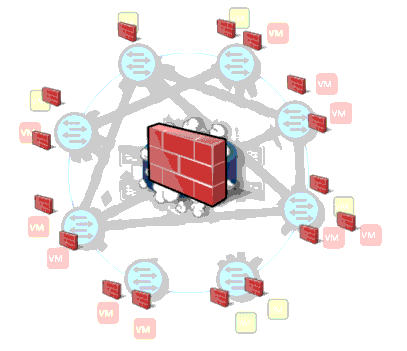
\includegraphics[width=1.0\textwidth]{dfw.png}
            \end{column}
            \begin{column}{0.5\textwidth}
                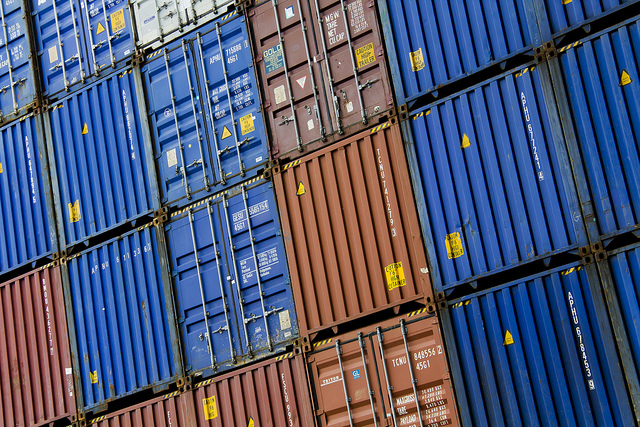
\includegraphics[width=1.0\textwidth]{containers.jpg}
            \end{column}
        \end{columns}
        %\blfootnote{%
        %    \tiny\url{http://www.routetocloud.com/2015/04/nsx-distributed-firewall-deep-dive/}}
        %\blfootnote{%
        %    \tiny\url{https://www.flickr.com/photos/lukeprice88/9703431992}}
        %\begin{itemize}
        %    \item Intelligent edge \bigskip
        %    \item Containers \medskip
        %\end{itemize}
    \end{frame}

    %\begin{frame}{}
    %    ``BPF has actually been really useful, and the real power of it is how
    %    it allows people to do specialized code that isn't enabled until asked
    %    for. Things like tracing and statistics (and obviously network
    %    filters) are prime examples of things where people want to do
    %    localized things for one particular machine (or one particular site)
    %    that aren't of the `everybody wants the same thing' kind. And that's
    %    where the whole dynamic `build a small program for it and attach it to
    %    xyz' comes in really useful.''
    %    \\[5pt]
    %    \rightline{{\rm --- Linus Torvalds%
    %        \blfootnote{{\tiny\url{https://www.zdnet.com/article/linus-torvalds-talks-about-coming-back-to-work-on-linux/}}}}}
    %\end{frame}

    \section{Socket-based firewalling}

    \begin{frame}{If we're co-located with the sockets~\ldots}
        %\begin{flushleft}
	%    If we're co-located with the sockets~\ldots \medskip
        %\end{flushleft}
        %\begin{center}
	%    \ldots~and we know the traffic is local~\dots \medskip
        %\end{center}
        \begin{flushright}
            \ldots~why build our own connection table? \medskip
        \end{flushright}
	\begin{center}
        %\includegraphics[width=0.8\textwidth]{keanu.png}
        
\includegraphics[width=0.6\textwidth]{mindblown.png}
	\end{center}
    \end{frame}

    \begin{frame}[fragile]{Socket table as a connection tracker}
        \centering
        \vfill
        \includesvg[width=0.8\textwidth]{sfw-sk-policy.svg}
%        \begin{verbatim}
%      +-+    +--------------+    +--------------+
%+-----+      |    Socket    |    |    Policy    |
%| NIC +------>    Table     +---->              +---->
%+-----+      +--------------+    +--------------+
%        \end{verbatim}
        \vfill
    \end{frame}

    \begin{frame}[fragile]{Socket safety}
        \begin{itemize}
            \item Sockets are reference-counted internally \smallskip
            \begin{itemize}
                \item Some memory-management under RCU rules \medskip
            \end{itemize}
            \item \verb+BPF_PROG_TYPE_CGROUP_SOCK+ \smallskip
            \begin{itemize}
                \item Access safety via reference held across BPF execution \medskip
                \item Bounds safety provided via bounds access checker \medskip
            \end{itemize}
            \item Packet hooks may execute before associated socket is known \medskip
            \begin{itemize}
                \item Need to handle reference counting \medskip
            \end{itemize}
        \end{itemize}
    \end{frame}

    \newsectionpage{Extending the BPF verifier}

    %\begin{frame}{Building socket-aware BPF programs}
    %    \begin{itemize}
    %        \item Safety \medskip
    %        \item Performance \medskip
    %        %\item Namespacing \medskip
    %        %\item Socket identity \medskip
    %        \item Metadata \medskip
    %    \end{itemize}
    %\end{frame}

    \begin{frame}{}
        \centering
        \vfill
        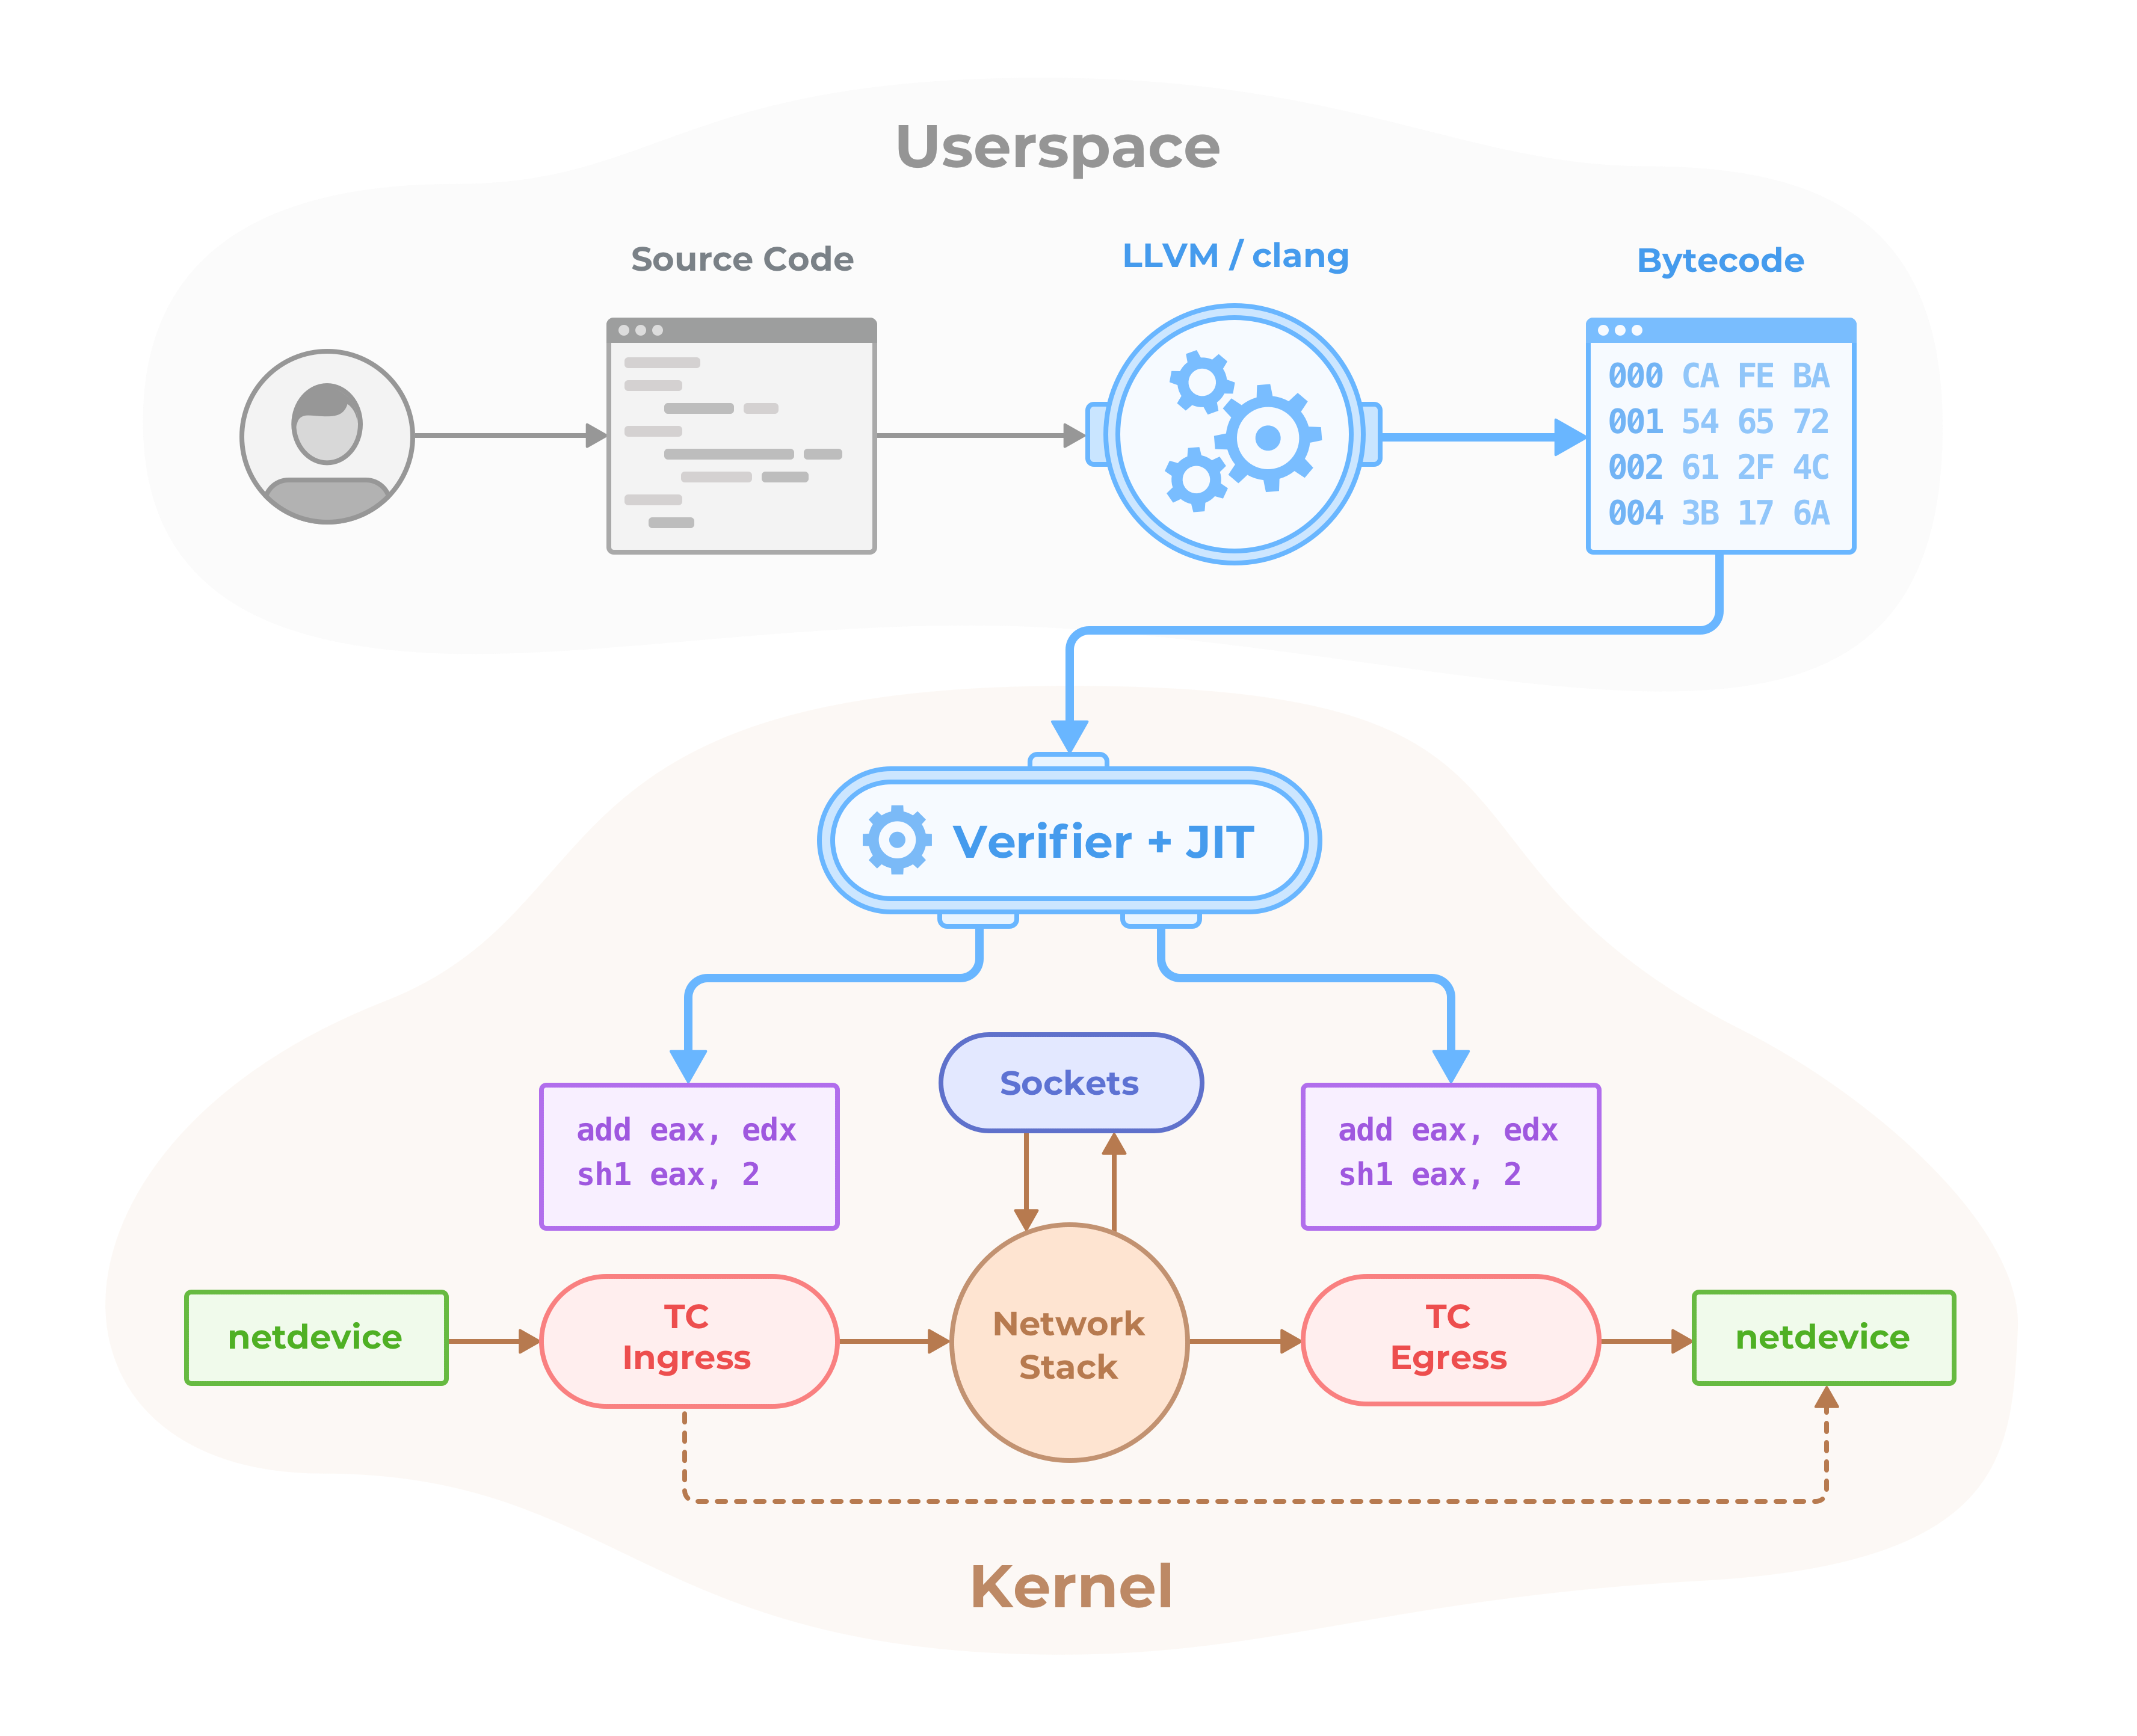
\includegraphics[width=0.8\textwidth]{verifier.png}
    \end{frame}

    \begin{frame}[fragile]{BPF verifier: Recap}
	\begin{itemize}
	    \item At load time, loop over all instructions \smallskip
            \begin{itemize}
                \item Validate pointer access \medskip
                \item Ensure no loops \medskip
                \item \ldots \medskip
            \end{itemize}
            \item Access memory out of bounds? \bigxmark \medskip
            \item Returns pointers it shouldn't? \bigxmark \medskip
            \item Everything safe? \bigcmark \medskip
	\end{itemize}
    \end{frame}

    \begin{frame}[fragile]{Socket reference counting}
        \begin{columns}[c]
            \hspace{0.02\textwidth}
            \begin{column}{0.46\textwidth}
            \begin{center}
            Implicit \bigskip
            \end{center}
            \verb+struct bpf_sock *sk;+\\
            ~\\
            \verb+sk = bpf_sk_lookup(+\ldots\verb+);+\\
            \verb+if (sk) {+\\
            ~~~~\ldots\\
            \verb+}+\\
            \verb+/* Kernel will free `sk' */+\\
            \end{column}
            %\hspace{-50pt}
            \hspace{0.02\textwidth}
            \vrule{}
            \hspace{0.02\textwidth}
            \begin{column}{0.46\textwidth}
            \begin{center}
            Explicit (mainline) \bigskip
            \end{center}
            \verb+struct bpf_sock *sk;+\\
            ~\\
            \verb+sk = bpf_sk_lookup(+\ldots\verb+);+\\
            \verb+if (sk) {+\\
            ~~~~\ldots\\
            ~~~~\verb+bpf_sk_release(sk);+\\
            \verb+}+\\
            \end{column}
            \hspace{0.02\textwidth}
        \end{columns}
    \end{frame}

    \begin{frame}{Reference counting in the BPF verifier}
        \begin{enumerate}
            \item Resource acquisition \bigskip
            \item Execution paths while resource is held \bigskip
            \item Resource release \bigskip
        \end{enumerate}
    \end{frame}

    \begin{frame}{Reference Acquisition}
        \begin{itemize}
            \item Generate an identifier \bigskip
            \item Store the identifier in the verifier state \bigskip
            \item Associate the register with the identifier \bigskip
        \end{itemize}
    \end{frame}

    \begin{frame}[fragile]{Reference misuse}
        \begin{itemize}
            \item Mangle and release \bigskip
            \item \verb+bpf_tail_call()+ \bigskip
            \item \verb+BPF_LD_ABS+, \verb+BPF_LD_IND+ \bigskip
        \end{itemize}
    \end{frame}

    \begin{frame}{Reference release}
        \begin{itemize}
            \item Validation of pointers \bigskip
            \item Remove identifier reference from state \bigskip
            \item Unassociate register identifier associations \bigskip
        \end{itemize}
    \end{frame}

    \newsectionpage{Extending the BPF API}

    \begin{frame}[fragile]{Simplest form}
        \begin{itemize}
            \item \verb+struct bpf_sock *bpf_sk_lookup(struct sk_buff *);+ \bigskip
            \item \verb+void bpf_sk_release(struct bpf_sock *);+ \bigskip
        \end{itemize}
    \end{frame}

    %\begin{frame}{Considerations for the API}
    %    \begin{itemize}
    %        \item Network Namespaces \bigskip
    %        \item Arbitrary socket lookup \bigskip
    %        \item Extensibility \bigskip
    %        \item Performance \bigskip
    %    \end{itemize}
    %\end{frame}

    \begin{frame}[fragile]{Namespaces}
        %\begin{itemize}
        %    \item Container orchestration from root netns \bigskip
        %    \item Container workload in child netns \bigskip
        %\end{itemize}
        \vfill
        \centering
        \includesvg[width=0.8\textwidth]{sk-lookup-netns.svg}
%        \begin{verbatim}
%+----------------------------------------+
%|                 +--------------------+ |
%|                 | +------+  +------+ | |
%|                 | |      |  |      | | |
%|                 | |  c1  |  |  c2  | | |
%|                 | |      |  |      | | |
%|                 | +------+  +------+ | |
%|    +--------+   |  +--+  Pod         | |
%|    | netdev |   |  |  |              | |
%|    +----+---+   +--+-++--------------+ |
%|         |            |                 |
%|     +---+------------++                |
%|     |     Bridge      |         Host   |
%|     +---+-------------+                |
%|         |                              |
%+---------+------------------------------+
%\end{verbatim}
        \vfill
    \end{frame}

    \begin{frame}{Arbitrary socket lookup}
        \begin{itemize}
            \item Use any tuple for lookup \bigskip
            \item Ease API across clsact, XDP \bigskip
            \item Simplify packet mangle and lookup \bigskip
        \end{itemize}
    \end{frame}

    \begin{frame}[fragile]{Extensibility}
        \begin{itemize}
            \item Allow influencing lookup behaviour \smallskip
            \begin{itemize}
                \item \verb+SO_REUSEPORT+ \bigskip
            \end{itemize}
            \item Determine socket type support at load time \smallskip
            \begin{itemize}
                \item Socket type supported? Load the program \medskip
                \item Not supported? Reject the program \bigskip
            \end{itemize}
        \end{itemize}
    \end{frame}

    \begin{frame}{Optimizations}
        \begin{itemize}
            \item Avoid reference counting \bigskip
            \item Allow lookup using direct packet pointers \bigskip
        \end{itemize}
    \end{frame}

    \begin{frame}[fragile]{Socket lookup API}
        \verbatiminput{../sk-lookup-api.h}
    \end{frame}

    \begin{frame}[fragile]{Socket lookup structures}
        \verbatiminput{bpf-tuple.h}
    \end{frame}

    \begin{frame}[fragile]{Socket structure}
        \verbatiminput{bpf-sock.h}
    \end{frame}

    \newsectionpage{Epilogue}

    \begin{frame}{Use case: Network devices}
        \begin{itemize}
	    \item Socket lookup from XDP \bigskip
            \item Management traffic? Send up the stack \bigskip
            \item Other traffic? Forward, route, load-balance \bigskip
        \end{itemize}
    \end{frame}

    \begin{frame}{Future work}
        \begin{itemize}
            \item More socket attribute access \bigskip
            \item Associate metadata with sockets \bigskip
            \item More uses for reference tracking \bigskip
                % Spin-locks, RCU
        \end{itemize}
    \end{frame}

    \section{}
    \begin{frame}{Thank you}
        \vfill
	\centering
	Joe Stringer \\\medskip
	joe@cilium.io
	\vfill
    \end{frame}

    %\begin{frame}{Thank you!}
    %    \begin{columns}[c]
    %        \begin{column}{0.3\textwidth}
    %            \vfill
    %            \centering
    %    	https://cilium.io/ \\\bigskip
    %    	@ciliumproject \\
    %            %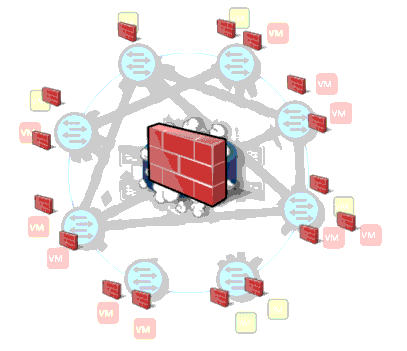
\includegraphics[width=1.0\textwidth]{dfw.png}
    %            \vfill
    %        \end{column}
    %        %\hspace{-50pt}
    %        %\vrule{}
    %        \begin{column}{0.7\textwidth}
    %            \vfill
    %            \centering
    %            Joe Stringer\\\bigskip
    %            joe@cilium.io\\
    %            %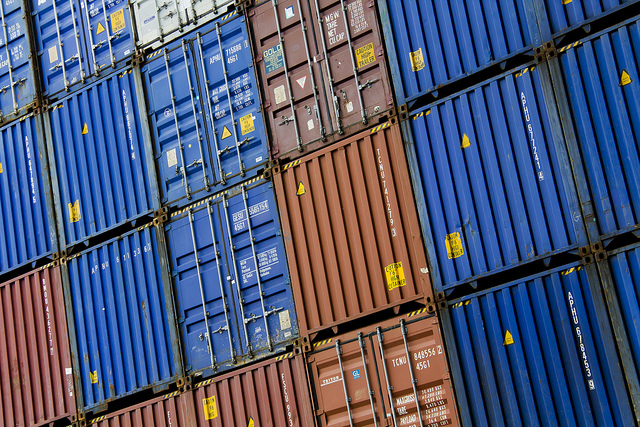
\includegraphics[width=1.0\textwidth]{containers.jpg}
    %            \vfill
    %        \end{column}
    %    \end{columns}
    %\end{frame}

\end{document}
